\chapter{Revisão da Literatura}\label{arte}


\section{Introdução}\label{arte:intro}

Nesse estudo, foi realizada uma revisão teórica e de pesquisas contemplando três campos, a saber: 
  \begin{itemize}
    \item O primeiro diz respeito aos modelos preditivos de mineração de dados relacionados à pesquisa em lide;
    \item O segundo relacionado às tecnologias mineração em textos de redes sociais;
    \item Finalmente o último campo de pesquisa relacionado às tecnologias de mapeamento através de sistemas de posicionamento global 
    aplicados ao sistema rodoviário.
  \end{itemize}


  
\section{CRISP-DM}

O ``CRoss Indrustry Standard Process for Data Mining'' -- CRISP-DM é um processo de mineração de dados que descreve como especialistas 
nesse campo aplicam as técnicas de mineração para obter os melhores resultados \cite{Crisp2000}.
O CRISP-DM é um processo recursivo, onde cada etapa deve ser revista até quando o modelo apresentar os resultados satisfatórios, preliminarmente definidos.
O Analista de Dados ou o Cientista de Dados é o profissional que acompanha e executa o processo.

O CRISP-DM foi concebido, desenvolvido e refinado através de ``workshops'' entre 1996 e 1999 \cite{Crisp2000}, por três entidades empresariais europeias que 
formavam um consórcio, tendo com parceiros a Daimler-Chrysler AG (Alemanha), que estava, à época, à frente da maioria das organizações empresariais e comerciais 
na aplicação de mineração de dados em seus negócios; 
a SPSS Inc.(EUA), que provê serviços baseados em mineração de dados desde 1990, tendo lançado o primeiro workbench de mineração 
de dados comerciais o Clementine®; 
e a NCR Systems Engineering Copenhagen (EUA e Dinamarca), com o Teradata®, uma Datawarehouse que estabelecia equipes de consultores especialistas em mineração 
de dados para atender a seus clientes. Hoje mais de 300 empresas contribuem para o modelo de processo CRISP-DM.

\subsection{Contexto de aplicação do CRISP -- DM}

O contexto da aplicação do CRISP-DM \cite{Crisp2000} é guiado desde o nível mais genérico até o nível mais 
especializado, sendo normalmente explicado em quatro dimensões:

\begin{itemize}
 \item O domínio da aplicação -- a área específica que o projeto de mineração de dados acontece;
 \item O tipo de problema -- descreve as classes específicas do objetivo do projeto de mineração de dados;
 \item Os aspectos técnicos -- cobrem as questões específicas como os desafios usualmente encontrados durante o processo de mineração de dados; 
 \item As ferramentas e técnicas -- dimensão específica que cada ferramenta/técnica de mineração de dados é aplicada durante o projeto.
\end{itemize}

A tabela abaixo sumariza e exemplifica essas dimensões no contexto de aplicação do CRISP-DM.

\begin{table}[!ht]

\caption{Mineração de dados -- contexto de aplicação \cite{Crisp2000}}
\vspace{1mm}
\centering
\begin{tabular}{c|c|c|c|c}
\textbf{Dimensão} & \textbf{Domínio da} & \textbf{Tipo de } & \textbf{Aspecto } & \textbf{Ferramentas } \\
		  & \textbf{aplicação}  & \textbf{Problema} & \textbf{técnico}  & \textbf{e Técnicas}   \\ \hline
\textbf{Exemplo}  & Modelo de           & Descrição e       & Dados             & Clementine  \\
                  & resposta            & sumarização       & faltantes         &             \\ \hline
      --- 	  & Predição            & Segmentação       & \textit{Outlies}  & MineSet     \\
         	  & agitada             &                   &                   &             \\ \hline
      ---         & ---                 & Descrição do      & ---               & Árvore de   \\
                  &                     & conceito          &                   & decisão     \\ \hline
      ---         & ---                 & Classificação     & ---               & ---         \\ \hline
      ---         & ---                 & Predição          & ---               & ---         \\ \hline
      ---         & ---                 & Análise de        & ---               & ---         \\
                  &                     & dependências      &                   & \\            
\\
\end{tabular}
\tiny Fonte: CRISP-DM -- 1.0
\end{table}


A aplicação das técnicas de mineração de dados identifica padrões ocultos nos dados, inacessíveis pelas técnicas tradicionais,
como por exemplo, consultas em banco de dados, técnicas estatísticas, dentre outras. Além disso, possibilita analisar um grande número de 
variáveis simultaneamente, o que não acontece com o cérebro humano \cite{possas1998data}, bem como, com outras técnicas. 
A análise desse processo permite extrair novos conhecimentos a partir dos dados, que é tratado na literatura como 
KDD -- Knowledge Discovery Database \cite{FayyadUeoutros}. Fayyad destaca a natureza interdisciplinar do KDD que contempla a intersecção 
de campos de pesquisa tais como Aprendizagem de Máquina (Machine Learning), Reconhecimento de Padrões, I.A., estatística, computação de alto 
desempenho e outros, propõe que o objetivo principal é extrair um conhecimento de alto nível a partir de dados de baixo nível num contexto de 
grandes bases de dados.
O CRISP-DM, por sua vez, engloba todos esses elementos como pode ser visto na figura a seguir:

\begin{figure}[!ht]
\centering
\caption{Domínio das técnicas aplicadas a mineração de dados}
\vspace{1mm}
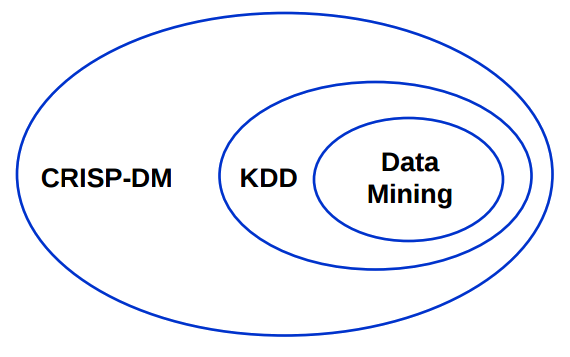
\includegraphics[width=60mm, height=20mm]{Figuras/BigData/RelacaoCrispKddDm.png}\\
\tiny Fonte: Neurotech -- 2012
\end{figure}

\pagebreak

\subsection{Ciclo de vida do CRISP--DM}

Um projeto de mineração de dados, na perspectiva do CRISP--DM, tem um ciclo de vida compreendido em seis fases:

A primeira, chamada \textbf{Entendimento do negócio}, é uma fase crucial da mineração, em que um especialista (ou muitos) deve ser consultado. 
O analista de dados consegue fazer re-uso de conhecimento lendo periódicos e artigos, mas a experiência de um profissional da área 
é condição ``sine qua non'' nessa fase.

Em seguida, o analista de dados passa à fase dois, \textbf{Entendimento dos dados}. Nessa fase o analista ``olha'' para os dados com a acurácia de um especialista, 
procurando identificar qualidade nos dados. Dados ausentes -- ``missing data'' -- são comuns em bases de dados não estruturadas, configurando-se como
um problema a ser considerado, pois seu tratamento pode consumir muito tempo do analista de dados. 

A terceira fase, \textbf{Preparação dos dados}, diz respeito à construção final do conjunto de dados. 
Preparar os dados significa criar e selecionar atributos, criar tabelas ou planilhas e registros dos dados.

Na quarta fase, \textbf{Modelagem de I.A.}, a tecnologia deve ser escolhida de forma criteriosa, baseada na experiência do analista de dados. 
Em sistemas de suporte à decisão, uma tecnologia inadequada pode levar a decisões imprecisas. É comum retornar às fases anteriores para adequar a técnica aos dados. 
Um modelo de regressão logística para problemas binários, redes neurais para problemas de classificação, e assim por diante.

Na fase cinco, \textbf{Avaliação de desempenho}, um ou muitos modelos devem ter sido construídos e testados, 
de forma que seja possível atingir uma alta qualidade do ponto de vista da análise dos dados, ou seja, que o 
modelo proposto esteja de adequado aos objetivos do negócio. Para tal é preciso que antes do desenvolvimento final 
do modelo, os passos executados até então sejam avaliados e revistos.

A sexta e última fase, caracteriza-se pela conclusão do modelo. No entanto a criação do modelo não é o fim do processo.
O conhecimento adquirido precisa ser incrementado, organizado e apresentado de maneira que o cliente possa usá-lo.
É importante ressaltar que este ciclo poderá ser retomado até que o modelo esteja adequado às necessidades e especifidades do cliente.

A figura a seguir ilustra as fases do ciclo:

\begin{figure}[!ht]
\centering
\caption{O padrão CRISP-DM \cite{Crisp2000}}
\vspace{1mm}
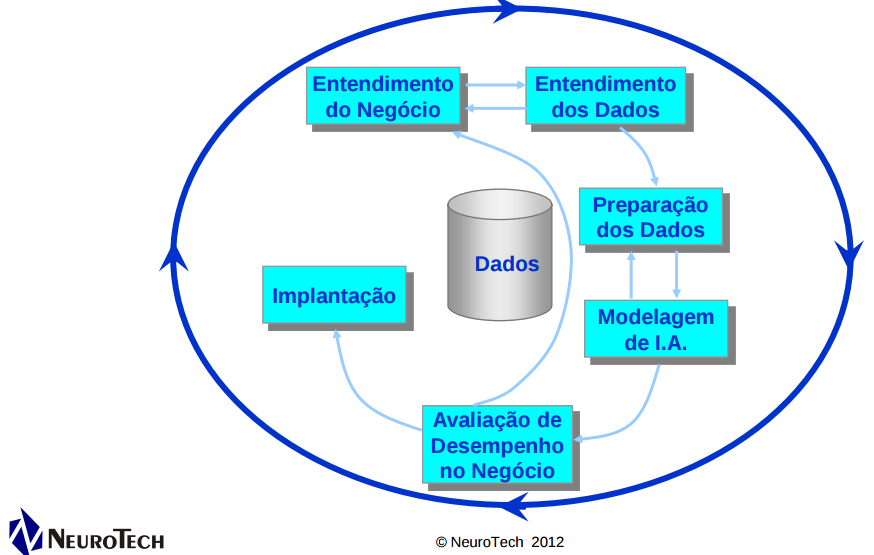
\includegraphics[width=70mm, height=70mm]{Figuras/BigData/CrispDM.png}\\
\tiny Fonte: CRISP-DM 1.0
\end{figure}




\pagebreak


\section{Mineração de dados}

A mineração de dados é um passo do processo da extração de conhecimento (KDD), que se caracteriza pela descoberta de padrões e/ou comportamentos em grandes bases de dados, 
também conhecido como repositórios de dados \cite{FayyadUeoutros}.
Existem vários tipos de dados e informações nesses repositórios que podem ser minerados, contudo esses dados, inicialmente são selecionados e agrupados, a seguir passam por 
uma fase de preprocessamento, que consiste em tratá-los de forma a prepará-los para a mineração. Essa fase é de 
fundamental importância na estruturação dos dados, uma vez que em grandes volumes de dados, também conhecido ``Datawarehouse'', podem existir inconsistências, faltas (missing data) ou 
duplicidade e erros de informações.

Nesse sentido, as técnicas de mineração de dados trabalham com dados estruturados, preenchidos em sua totalidade sem \textit{missing data}, para poder extrair informações relevantes.
Existem várias maneiras de se contornar os dados ausentes, como o preenchimento dos dados através de técnicas de inteligência artificial, da média dos valores, quando dados numéricos 
ou com a moda, quando os dados forem categóricos. Para cada tipo de dados existem técnicas apropriadas para serem aplicadas sobre eles, algumas mais sensíveis às problemáticas elencadas anteriormente
e outras mais robustas \cite{DataMining2}, que por sua vez estão associadas a classes de problemas que a mineração trata, a tabela 2.1 delineou o domínio.
Isso será tratado na seção Aprendizagem de Máquina ou ``Machine Learning''.
O caminho da extração dos dados até sua mineração e extração de conhecimento é longa.
Na figura a seguir temos a ilustração desse caminho:

\begin{figure}[!ht]
\centering
\caption{Fases da mineração de dados até extração do conhecimento}
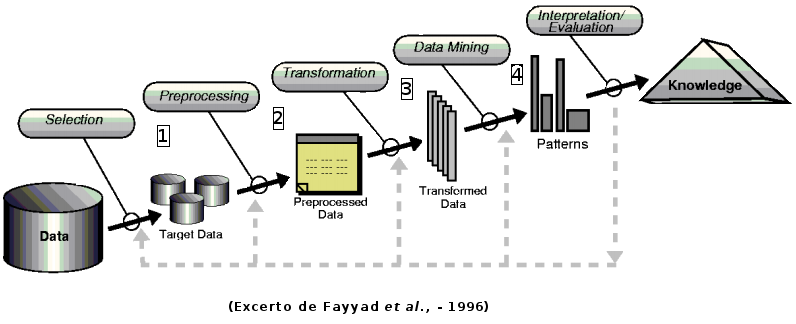
\includegraphics[width=135mm, height=65mm]{Figuras/BigData/FayyadSemFundo.png}
\end{figure}



A origem dos dados, os ``inputs'' estão representados na figura onde se lê ``Data'' este está repleto de \textit{missing data} e/ou dados inconsistentes, conhecidos como dados não estruturados. 
O balão onde se lê ``Selection'' representa a coleta das informações ou a seleção dos dados no \textit{Big Data}.
Em nossa pesquisa esses dados são provenientes das mais diversas fontes, tais como, redes sociais, câmaras de trânsito, informações de satélites meteorológicos e outras fontes.

Armazenar dados provenientes de redes sociais nessa etapa pode ser um grande problema, devido à sua extensão, porém os dados relevantes podem ser armazenados em ``Target Data'' 
com tecnologia apropriada, utilizando-se técnicas de ``Map'' e ``Reduce'' ou mineração de dados em textos para criar \textit{cluster} de informações e ler os fluxos de dados (stream data). 
Algumas técnicas de IA podem ser aplicadas nessa etapa como, [``Data Mininng Swarm Robotics'' através de Botnets \footnote{Botnet é citado no sentido da coleta de informações} ou ``Swarm Intelligence''. ]

No balão ``Preprocessing'' os dados não-estruturados são tratados, por exemplo, retirando os \textit{missing data}. 
Para estruturar as informações é preciso utilizar técnicas linguísticas, uma vez que existe lógica entre eles \cite{Aranha2006}.
Esses dados normalmente são coletados por técnicas de Mineração de Textos, também conhecidas como Mineração de Dados em Textos, técnicas de IA como ``Machine Learning'' 
têm sido muito utlizadas. Em ``Transformation'' os dados foram em estruturados, podendo ser armazenados em Bancos de Dados, conhecidos como Datawarehouse, por exemplo o Hive. 

O processo de Mineração dos dados começa no balão ``Data Mining'', onde são aplicadas as técnicas de IA conhecidas como classificadores, para extração de padrões, tais como: 
``Decision Tree'' (Árvore de decisão), ``Artificial Neural Network'' (Redes neurais artificiais), ``Logistic Regression'' (Regressão Logística) e ``Deep Learning''.
Algumas técnicas de mineração de dados são fortemente influenciadas pelas informações na entrada (input), como as Árvores de decisão \cite{DecisionTree}. 
As Redes Neurais, dependendo da quantidade de variáveis de entrada, paderão ter milhares de neurônios na camada intermediária, o que inviabilizaria essa metaheurística 
\footnote{Metaheurística são heurísticas aplicadas em problemas onde os custos computacionais não são tratáveis em tempo polionomial, devido às explosões combinatórias geradas
pelo grande número de tentativas. Metaheurísticas bioinspiradas metaforizam o comportamento de animais sociais, tais como formigas, pássaros, peixes e outros}.

Todas essas etapas descritas na figura são recorrentes, como indicam as setas pontilhadas que retornam aos passos anteriores.
Utilizar técnicas de mineração de dados, além de extrair dados, extrai conhecimento, com isso pode-se predizer os resultados futuros na saída do modelo, 
quando determinados dados ocorrem na entrada \cite{Amin2015a}, essa técnica de extração de conhecimento chama-se \textit{Knowledge Discovery Databases} (KDD).
O KDD utiliza métodos de Aprendizagem de Máquina para efetuar essa extração

\pagebreak

\section{Aprendizagem de Máquina}\label{arte:palavraChave:Machine}

Aprendizagem de Máquina ou ``Machine Learning'' são métodos para analisar dados de forma automatizada e interativa.
As técnicas algorítmicas apresentadas nas seções subsequentes são parte da grande família de algorítimos que compõem 
o aprendizado de máquina aplicado a mineração de dados.

As técnicas de mineração aplicadas na descoberta de conhecimento podem ser agrupadas de acordo com suas funcionalidades \cite{DataMining2}, 
essas funcionalidades tem como característica principal a maneira como são descobertos os padrões no dados, elas podem estar 
em uma das duas categorias: tarefas descritivas ou tarefas preditivas. As tarefas mineração descritivas preocupam-se nas características 
dos dados no conjunto de dados, o ``data set''. As tarefas de mineração preditivas induzem regras nos dados correntes para produzirem 
predições \cite{DataMining2}. A seção seguinte analisa as tarefas preditivas.

\subsection{Classificação e Regressão para análise preditivas}

Classificação é um processo para encontrar um modelo que descreve e distingue classes de dados. 
Esse modelo tem como base de análise um conjunto de treinamento (i.e. objetos de dados para os quais 
serão encontrados rótulos que os classifiquem). 
Esse modelo é usado para predizer quais rótulos de classes terão os objetos desconhecidos.
O modelo pode ser representado por regras de classificação do tipo ``IF - THEN'', por árvores de decisão, redes neurais e outros. 
Regras de classificação se distinguem de regras de indução da seguinte forma:
\begin{itemize}
 \item Uma regra de classificação poderia ser: $if$ L $them$ class = $C_{1}$ ou $if$ L $them$  $C_{1}$
 \item Uma regra de indução seria: $ if$ L $them$ R que por sua vez produz novas regras 
\end{itemize}

As árvores de decisão são estruturas como fluxogramas, possuem nós e ramificações, 
cada nó é um teste no valor do atributo como:\\
\\
  $age(X,``youth")$ AND $income(X,``high")  \to classe (X,``A")$\\
  $age(X,``youth")$ AND $income(X,``low") \to classe (X,``B")$\\
  $age(X,``middle-aged")$  $\to classe (X,``B")$\\
  $age(X,``senior")$       $ \to classe (X,``B")$\\

\pagebreak
  
A seguir, a árvore de decisão que explicita se um cliente, de acordo com sua idade terá determinada classe:
\begin{figure}[!ht]
\centering
\caption{Árvore de decisão}
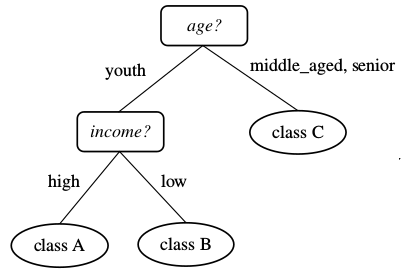
\includegraphics[width=60mm, height=55mm]{Figuras/BigData/arvorejovem.png}\\
\tiny Fonte: Han, J. and Kamber, M. 
\end{figure}  

A figura a seguir representa uma rede neural com as mesmas características da árvore de decisão anterior:
\begin{figure}[!ht]
\centering
\caption{Rede Neural}
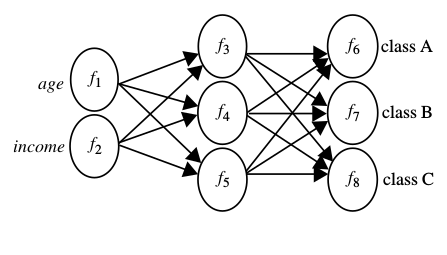
\includegraphics[width=85mm, height=55mm]{Figuras/BigData/redeneural.png}\\
\tiny Fonte: Han, J. and Kamber, M. 
\end{figure}  

As árvores de decisão produzem regras de indução, são algoritmos rápidos, contudo dados impuros podem comprometer o desempenho desse algoritmo. 
A fase de extração dos dados do é fortemente influenciáveis pelas variáveis escolhidas, \cite{DecisionTree} 
isso pode representar o desafio maior para implementar esta técnica. 

Outro problema que pode ser encontrado em algoritmos de aprendizagem é o ``overfitting'' ((( falar de overfitting)))

\pagebreak

\subsection{Árvore de Decisão}

Han e Kamber \cite{DataMining} definem indução por árvore de decisão como a aprendizagem de árvore de decisão a partir de classes rotuladas nas tuplas de treinamento. 
A estrutura da árvore de decisão é semelhante a um fluxograma, onde cada nó interno (não-folha) indica um teste de atributo, cada ramo representa o resultado de um teste e 
cada nó da folha possui um rótulo de classe. O nó de nível mais superior é chamado de nó-raiz.


Para Ian e Frank \cite{MachineLearning}, as árvores de decisão podem ser representadas por uma abordagem ``dividir para conquistar'' para resolução de problemas de 
aprendizagem, a partir de um conjunto de instâncias independentes. Os nós em uma árvore de decisão ``testam'' um atributo específico, comparando seu valor com uma constante.
No entanto, algumas árvores podem comparar dois atributos com outros ou utilizarem uma função para tal.
As árvores de decisão podem ser classificadas em dois tipos: árvores de regressão (regression trees), que são utilizadas para estimar atributos numéricos, e árvores de 
classificação (classification trees), usadas para análise de variáveis categóricas.

\pagebreak

\subsubsection{Tipos de Árvores de decisão}
O algorítimo \textit{C4.5} é considerado um exemplo clássico de método de indução de árvores de decisão. O \textit{C4.5} \cite{Learning2007} foi inspirado no algoritmo 
\textit{ID3} \cite{Learning1979}, que produz árvores de decisão a partir de uma abordagem recursiva de particionamento de um conjunto de dados, utilizando conceitos e medidas 
da Teoria da Informação \cite{TeoriaInf}.

As árvores de decisão têm uma característica peculiar, a saída do modelo de predição (o output), com regras se -- então é claramente perceptivel por analistas humanos.
Essa qualidade é utilizada para interpretar os resultados.


\subsection{Regressão}

\subsubsection{Tipos de regressão}

\subsubsection{Logística}
Regressão logística (linear, logística, ou outras) é uma técnica para analisar o relacionamento entre variáveis. No entanto, a regressão linear é utilizada para problemas de natureza
contínua, sendo que a regressão logística é semelhante, contudo, a variável dependente não é contínua, é discreta ou categórica \cite{DecisaoCredito}.

A regressão logística está definida como o logarítmo a seguir:

\begin{equation}
 log{\frac{\pi(x)}{1-\pi(x)}} = \beta_0 + \beta_1 x_1 + \beta_2 x_2 + ... + \beta_p x_p
\end{equation}

onde $\pi(x)$ é definido como:

\begin{equation}
 \pi(x) = \dfrac{1}{1 + e^{-{\beta_0 + \beta_1 x_1 + \beta_2 x_2 + ... + \beta_p x_p}}}
\end{equation}

e $x_1, x_2,..., x_p$ são as variáveis a serem exploradas.


A aplicação da regressão logística foi utilizada, pela primeira vez, com sucesso na oferta de crédito nos anos seguintes ao fim da 2ª guerra mundial, para tomar decisão 
de oferecer crédito a terceiros \cite{RegrecaoLog}.
A regressão logística é comumente aplicada para problemas de classificação binária (ou booleano).

\pagebreak

\subsection{Redes Neurais}

Uma rede neural artificial (RNA) é uma técnica que constrói um modelo matemático, baseado em funções, de um modelo
neural biológico simplificado, contudo este modelo tem capacidade de aprendizado, generalização, associação e abstração.

((( continuar )))

\subsubsection{Tipos de Redes Neurais}

\pagebreak


\subsection{Medida de desempenho e qualidade}

Quando são desenvolvidos sistemas de predição e análise de diagnóstico, avalia-se o desempenho e a qualidade dos resultados encontrados.
Um método gráfico eficiente para detecção e avaliação da qualidade de sinais, conhecido como \textit{Receiver Operating Characteristic} -- ROC, ou curva ROC \cite{ROC},
foi criado e desenvolvido na década de 50 do século passado, para avaliar a qualidade da transmissão de sinais em um canal com ruído.
Recentemente a curva ROC tem sido adotada em Mineração de dados e Aprendizagem de Máquina \cite{MD_AM}, em sistemas de suporte à decisão na medicina, para analisar a qualidade da detecção 
de um determinado teste bioquímico, na psicologia para detecção de estímulos \cite{Discriminativo} em pacientes, e na radiologia para classificação de imagens.

Essas métricas são amplamente utilizadas na classificação binária de resultados contínuos. Para isso ser construído utiliza-se a Matriz de Contingência que classifica as probabilidades como:
verdadeiro positivo, falso positivo, falso negativo e verdadeiro negativo, respectivamente \textit{True Positive -- TP, False Positive -- FP, False Negative -- FN e True Negative -- TN },
também conhecida como matriz de confusão, descrita na tabela a seguir:

%tabela 5
\begin{table}[ht]
\centering
\caption{Matriz de Confusão}
\vspace{1mm}
\begin{tabular}{l|c|c}
\hline
\textbf{} & \textbf{Predito} & \textbf{}\\
\hline
\textbf{Real}  & TP   FN & Positive -- POS\\
\textbf{Real}  & FP   TN & Negative -- NEG\\
\hline
   ---         & PP   PN &    ---         \\
\end{tabular}
\tiny Fonte: \cite{Bradley1997}
\end{table}

A matriz da Tabela 2.3 sintetiza a matriz da Tabela 2.4, portanto as duas tabelas são equivalentes.

%tabela 6
\begin{table}[ht]
\centering
\caption{Matriz modelo de Confusão}
\vspace{1mm}
\begin{tabular}{l|c|c}
\hline
\textbf{}           & \textbf{Y}     \textbf{$\bar{Y}$}   & \textbf{}\\
\hline
\textbf{X}          & P(X,Y)         P(X,$\bar{Y}$)       & Positive -- POS\\
\textbf{$\bar{X}$}  & P($\bar{X}$,Y) P($\bar{X},\bar{Y}$) & Negative -- NEG\\
\hline
   ---              & P(Y)           P($\bar{Y}$)         &     ---        \\
\end{tabular}
\tiny Fonte: \cite{Bradley1997}
\end{table}


De acordo com as probabilidades condicionais temos:

\begin{equation}
 P(X,Y) = P(X|Y).P(Y) = P(Y|X).P(X)
\end{equation}

Então, a taxa de verdadeiros positivos será $P(Y|X)$ e a probabilidade de falsos alarmes ou taxa de falsos positivos será $P(Y,\bar{Y})$, a barra sobrescrita em $\bar{X}$
(ou $\bar{Y}$) representa negação. \\
A curva ROC será construída cruzando-se a taxa dos verdadeiros positivos (tpr = P(Y|X)) com a taxa dos falsos positivos (fpr = P(Y,$\bar{X}$)).

\pagebreak

\section{Redes sociais}

As redes sociais são um arcabouço de informações sobre todo tipo de assunto vivenciado no cotidiano das pessoas, inclusive situações que dizem respeito ao nosso ambiente de pesquisa.
O cenário abaixo, encontrado numa rede social, exemplifica a sequência de informações retiradas do Twitter, um microblog onde os usuários escrevem num pequeno espaço (cerca de 140 caracteres), 
os mais diversos assuntos, e os usuários conectam por uma multiplicidade de dispositivos: computadores, tablets e celulares, formando uma grande rede social mundial. 
A ideia inicial do Twitter, segundo seus fundadores, era que essa rede se comportasse como um ``SMS da Internet'' \cite{Twitter2015}. 
As informações são enviadas aos usuários, conhecidas como twittes, em tempo real e também enviadas aos usuários seguidores que tenham assinado para recebê-las.

"Em 2010 empresas e usuários armazenaram mais de 13 exabytes de novos dados" \cite{bigdataQualquerUm}.

%tabela 5
\begin{table}[!ht]
\centering
\caption{Volume de dados no mundo}
\vspace{1mm}
\begin{tabular}{l|c|c|c}
\hline
\textbf{Ano} & \textbf{Qtd} & \textbf{Unidade} & \textbf{Múltiplo}\\
\hline
2000 & 800 & terabytes – TB & $10^{12}$\\
2006 & 160 & petabytes – PB & $10^{15}$\\
2009 & 500 & exabytes – EB & $10^{18}$ \\
2012 & 2,7 & zettabytes – ZB & $10^{21}$\\
2020 & 35 & yottabytes – YB & $10^{24}$\\
\end{tabular}
\end{table}



\pagebreak

A seguir pode-se verificar uma sequência de twittes da Polícia Rodoviária Federal de Santa Catarina:

\begin{figure}[ht]
\subfigure{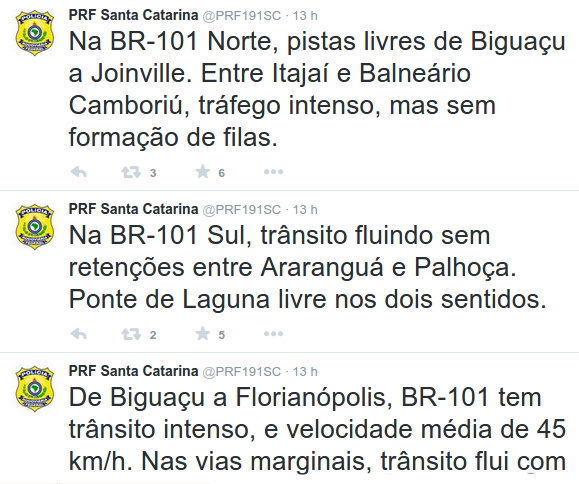
\includegraphics[width=60mm, height=48mm]{Figuras/BigData/twittePRF.png}}
\quad \quad \quad \quad
\subfigure{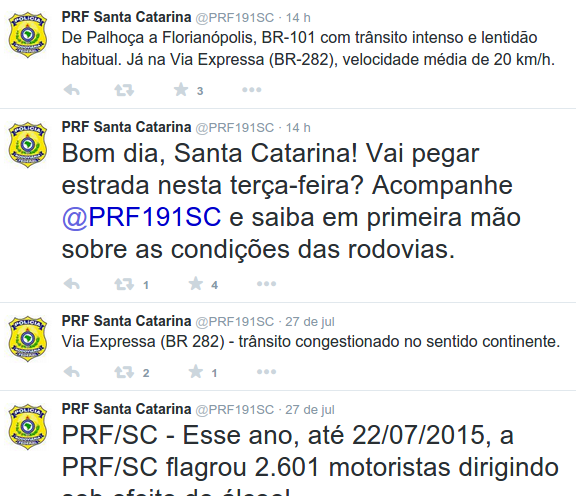
\includegraphics[width=60mm, height=48mm]{Figuras/BigData/twittePRF2.png}}
\end{figure}

A Polícia Rodoviária Federal de Santa Catarina, disponibilizou às 13h através do canal @PRF191SC, informações relevantes sobre o trânsito naquela localidade, 
num espaço temporal variado, por exemplo: entre Itajaí e Balneário Camboriú o transito está intenso. Isso sugere que a frota de caminhões deva ter uma
rota alternativa caso a situação persista por muito tempo. No primeiro twitte da segunda coluna, é informado em Via Expressa (BR 282) que o trânsito está lento com 
velocidade de 20km/h (praticamente congestionado). Essa informação sugere que deve ser pensada uma rota alternativa, caso o congestionamento persista por muito tempo.

Outra rede social conhecida pelos condutores de veículos é o Waze. O Waze é um aplicativo de navegação para o trânsito, funciona em aparelhos celulares e tablets. 
Os utilizadores desse aplicativo são conhecidos como wazers e compartilham informações sobre o trânsito, em tempo real. Toda via, as informações somente estão disponíveis 
no momento em que são postadas pelos utilizadores, por um período de tempo pequeno. Caso não haja usuários trafegando pelas vias ou caso os mesmos não tenham disponibilidade 
em postar informações, não há o que se compartilhar.
Outro problema levantado com o waze é que, caso não haja conexão à Internet não há como acessar os dados dos 'wazers', para navegação.

Além dos dados que chegam ao \textit{Big Data} através das redes sociais, as grandes cidades têm disponíveis câmeras de monitoramento do trânsito nos semáforos ou próximas a eles; 
algumas com cobertura por canais de televisão bem como câmaras de segurança próximos às rodovias, coletando informações em tempo real. 
Os dados desses dispositivos são gravados, sendo conhecidos como \textit{stream} de dados. 
Esses \textit{streams} podem ser disponibilizados na Internet, em sítios eletrônicos especialmente construídos para isso, como o http://vejoaovivo.com.br dentre outros.

Os dados disponibilizados pelos diversos meios de comunicação não estão em formato que possam ser utilizados imediatamente, precisando antes serem processados. 
Tais dados não processados são conhecidos como ``dados frios''. O processo de tratar as informações, retirando-lhes o ``lixo'' e transformando dados ``frios'' em dados 
``quentes'', é um processo que tem um custo temporal elevado, devido ao volume dos dados.



\pagebreak
\subsection{ Data Mining - Text Data Mining}\label{arte:palavraChave:DataMiningBigData}

Minerar dados em texto nas redes sociais não é uma tarefa atômica, devendo ser divida em várias etapas, com processos específicos em cada uma delas, como descrito anteriormente. 
Extrair conhecimento dos dados não processados não faz sentido, tratá-los apenas ``per si'' exige muito trabalho de IA, como Mineração de dados em textos. 
A Mineração em textos é inspirada em técnicas de ``Machine Learning'' \cite{Aranha2006}. 
Contudo analisar textos é basicamente entender o significado do texto, baseado em regras de associação lógica.
O mapa mental a seguir mostra um modelo de análise de texto feito por seres humanos.

\begin{figure}[htpb]
\centering
\caption{Mapa mental da Mineração em textos}
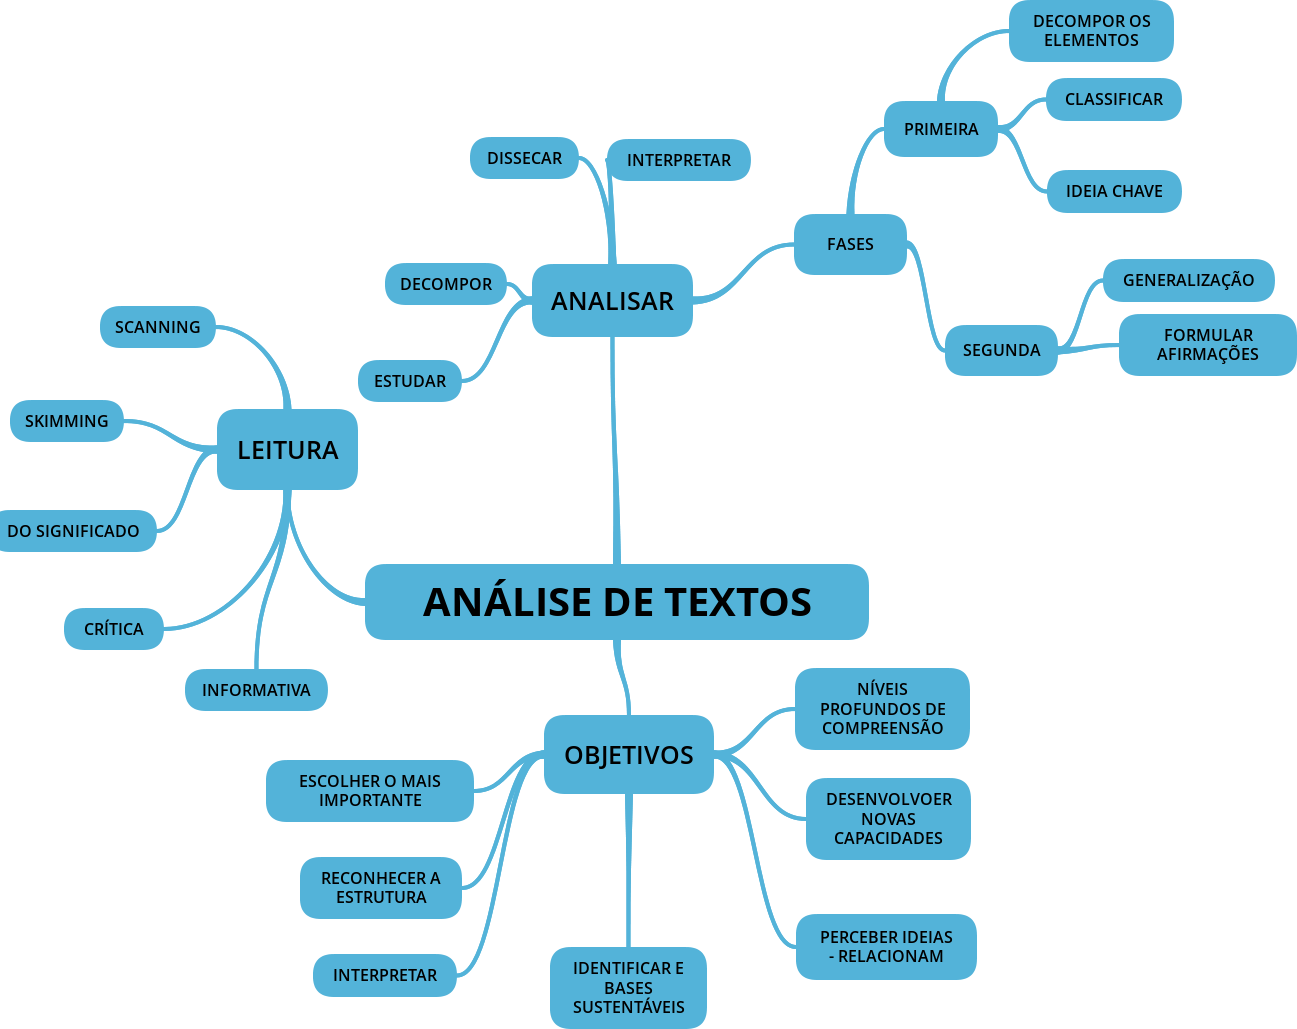
\includegraphics[width=120mm, height=60mm]{Figuras/BigData/Analise_Textos.png}
\end{figure}
